\documentclass[letterpaper,12pt,oneside,final]{book}
%%
%%  Gabarit bilingue de mémoire de maîtrise ou thèse de doctorat.
%%  Bilingual template for dissertations and theses @ Polytechnique Montreal.

%%  Normalement, il n'est pas nécessaire de modifier ce document
%%  sauf pour établir le langage (français ou anglais) et pour changer les noms des fichiers à inclure.
%%  Usually, this document needs to be modified only to set up the language (French or English) and to change the names of the files to include.
%%
%%  Version: 2022-06-7
%%
%% Accepte les caractères accentués dans le document (UTF-8).
%% Supports accented characters in the document (UTF-8).


\makeatletter
\def\bstctlcite{\@ifnextchar[{\@bstctlcite}{\@bstctlcite[@auxout]}}
\def\@bstctlcite[#1]#2{\@bsphack
 \@for\@citeb:=#2\do{%
   \edef\@citeb{\expandafter\@firstofone\@citeb}%
   \if@filesw\immediate\write\csname #1\endcsname{\string\citation{\@citeb}}\fi}%
 \@esphack}
\makeatother

%% LA COMMANDE SUIVANTE ÉTABLIT LE LANGAGE DE LA THÈSE : ÉCRIRE french POUR UNE THÈSE EN FRANÇAIS
%% THE NEXT COMMAND DETERMINES THE LANGUAGE OF THE THESIS: WRITE english FOR A THESIS IN ENGLISH
\newcommand\Langue{french}            

\usepackage{ifthen}
\usepackage[utf8]{inputenc}
%%
%% Support pour l'anglais et le français (français par défaut).
%% Support for English and French (French by default).

%\usepackage[cyr]{aeguill}
\usepackage{lmodern}      % Police de caractères plus complète et généralement indistinguable visuellement de la police standard de LaTeX (Computer Modern). / A more complete and generally visually indistinguishable font from the standard LaTeX font (Computer Modern).
\usepackage[T1]{fontenc}  % Bon encodage des caractères pour qu'Acrobat Reader reconnaisse les accents et les ligatures telles que ffi. / Good character encoding so that Acrobat Reader recognizes accents and ligatures such as ffi.

\ifthenelse{\equal{\Langue}{english}}{
	\usepackage[french,english]{babel}
}{
	\usepackage[english,french]{babel} 
}

%%
%% Charge le module d'affichage graphique. / Loads the graphics package.
\usepackage{graphicx}
\usepackage{epstopdf}  % Permet d'utiliser des .eps avec pdfLaTeX. / Allows using .eps with pdfLaTeX.
%%
%% Recherche des images dans les répertoires. / Search for images in folders.
\graphicspath{{./images/}{./dia/}{./gnuplot/}}
%%
%% Un float peut apparaître seulement après sa définition, jamais avant. / A float can appear only after its definition, never before.
\usepackage{flafter,placeins}
%%
%% Autres modules. / Other packages.
\usepackage{amsmath,color,soulutf8,longtable,colortbl,setspace,xspace,url,pdflscape,cite}
%%
%% Support des acronymes. / Support for acronyms.
\usepackage[nolist]{acronym}
\onehalfspacing                % Interligne 1.5. / Line spacing = 1.5.
%%
%% Définition d'un style de page avec seulement le numéro de page à
%% droite. On s'assure aussi que le style de page par défaut soit
%% d'afficher le numéro de page en haut à droite. / Definition of a page 
%% style with only the page number on the right. We also make sure that the 
%% default page style is to display the page number at the top right.
\usepackage{fancyhdr}
\fancypagestyle{pagenumber}{\fancyhf{}\fancyhead[R]{\thepage}}
\renewcommand\headrulewidth{0pt}
\makeatletter
\let\ps@plain=\ps@pagenumber
\makeatother
%%
%% Module qui permet la création des bookmarks dans un fichier PDF. / Package that allows the creation of bookmarks in a PDF file.
%\usepackage[dvipdfm]{hyperref}
\usepackage{hyperref}
\usepackage{caption}  % Hyperlien vers la figure plutôt que son titre. / Hyperlink to the figure rather than its title.
\makeatletter
\providecommand*{\toclevel@compteur}{0}
\makeatother

%% Modules ajoutés (2022) / packages added (2022)
\usepackage{subcaption} % figures & sous figures / figures & subfigures
\usepackage{siunitx} % unites SI / SI units
\usepackage{amssymb} % autres symboles mathematiques / other mathematical symbols
\usepackage[bottom]{footmisc} % pour avoir les notes de bas de page en dessous des figures... / to have the footnotes below the figures
%\usepackage{listings} % Si on veut ajouter des lignes de codes dans le texte / If you want to add lines of code to the text


%%
%% Définitions spécifiques au format de rédaction de Poly.
%% Here we define the Poly formatting.
\RequirePackage[\Langue]{MemoireThese}
%%
%% Définitions spécifiques à l'étudiant.
%% Student-specific definitions.
%% -----------------------------------
%% ---> À MODIFIER PAR L'ETUDIANT / TO BE MODIFIED BY THE STUDENT <---
%% -----------------------------------
%%
%% Commandes qui affichent le titre du document, le nom de l'auteur, etc.
% Commands that display the document title, the author's name, etc.
\newcommand\monTitre{Titre de mon document / Title }
\newcommand\monPrenom{Christine}
\newcommand\monNom{Perron}
\newcommand\monDepartement{génie informatique et génie logiciel}  % Department
\newcommand\maDiscipline{Génie informatique}
\newcommand\monDiplome{D}        % (M)aîtrise ou (D)octorat / (M)aster or Ph(D)
\newcommand\anneeDepot{2019}    % Year
\newcommand\moisDepot{Janvier}       % Month
\newcommand\monSexe{F}           % "M" ou "F" = Gender
\newcommand\PageGarde{N}         % "O" ou "N" = Yes or No
\newcommand\AnnexesPresentes{O}  % "O" ou "N". Indique si le document comprend des annexes. / If the thesis includes annexes = O; if it does not N = No.
\newcommand\mesMotsClef{Liste,de,mot-clés,séparés,par,des,virgules}
%%
%%  DEFINITION DU / OF JURY
%%
%%  Pour la définition du jury, les macros suivantes sont definies: / For the definition of the jury, the following macros are defined:
%%  \PresidentJury, \DirecteurRecherche, \CoDirecteurRecherche, \MembreJury, \MembreExterneJury
%%
%%  Toutes les macros prennent 3 paramètres: Sexe (M/F), Nom, Prénom
%%  All the macros have 3 parameters: Gender (M/F), Last name, First name
\newcommand\monJury{\PresidentJury{F}{Dubois}{Danielle}\\
\DirecteurRecherche{M}{Vigot}{Sébastien}\\
\CoDirecteurRecherche{F}{Couture}{Marie}\\
\MembreJury{M}{Tremblay}{Jean}\\
\MembreExterneJury{M}{Brown}{Joseph}}


\ifthenelse{\equal{\monDiplome}{M}}{
\newcommand\monSujet{Mémoire de maîtrise}
\newcommand\monDipl{Maîtrise ès sciences appliquées}
}{
\newcommand\monSujet{Thèse de doctorat}
\newcommand\monDipl{Philosophi\ae{} Doctor}
}
%%
%% Informations qui sont stockées dans un fichier PDF.
%% Information that is stored in a PDF file.
\hypersetup{
  pdftitle={\monTitre},
  pdfsubject={\monSujet},
  pdfauthor={\monPrenom{} \monNom},
  pdfkeywords={\mesMotsClef},
  bookmarksnumbered,
  pdfstartview={FitV},
  hidelinks,
  linktoc=all
}

%% Ajoute en 2022 (ajout des titres complets des tables et figure et alignement)
%% Added in 2022 (added full table and figure titles and alignment)
\usepackage[titles]{tocloft}
  \renewcommand{\cftchapleader}{\cftdotfill{\cftsecdotsep}} % dotted chapter leaders

\renewcommand\cfttabindent{0pt}
\renewcommand\cfttabnumwidth{7em}
\renewcommand\cfttabpresnum{\tablename\ }

\renewcommand\cftfigindent{0pt} 
\renewcommand\cftfignumwidth{7em}
\renewcommand\cftfigpresnum{\figurename\ }

\ifthenelse{\equal{\Langue}{english}}{
	\renewcommand\cftchapfont{CHAPTER }
    \renewcommand\cftchappagefont{}
}{
	\renewcommand\cftchapfont{CHAPITRE }
    \renewcommand\cftchappagefont{}
}
%

%%
%% Il y a un document par chapitre du mémoire ou thèse.
%% There is one document per chapter of the thesis or dissertation.

\begin{document}
\bstctlcite{IEEEexample:BSTcontrol}

%%
%% Page de titre du mémoire ou de la thèse.
%% Title page of the dissertation or thesis.
\frontmatter
%% Compte optionellement la page de garde dans la pagination.
%% Optionally counts the cover page in the pagination.
\ifthenelse{\equal{\PageGarde}{O}}{\addtocounter{page}{1}}{}
\thispagestyle{empty}%
\begin{center}%
\vspace*{\stretch{0.1}}
\textbf{POLYTECHNIQUE MONTRÉAL}\\
affiliée à l'Université de Montréal\\
\vspace*{\stretch{1}}
\textbf{\monTitre}\\
\vspace*{\stretch{1}}
\textbf{\MakeUppercase{\monPrenom~\monNom}}\\
Département de~{\monDepartement}\\
\vspace*{\stretch{1}}
\ifthenelse{\equal{\monDiplome}{M}}{Mémoire présenté}{Thèse présentée} en vue de l'obtention du diplôme de~\emph{\monDipl}\\
\maDiscipline\\
\vskip 0.4in
\moisDepot~\anneeDepot
\end{center}%
\vspace*{\stretch{1}}
\copyright~\monPrenom~\monNom, \anneeDepot.
%%
%% Identification des membres du jury.
%% Jury members.
\newpage\thispagestyle{empty}%
\begin{center}%

\vspace*{\stretch{0.1}}
\textbf{POLYTECHNIQUE MONTRÉAL}\\
affiliée à l'Université de Montréal\\
\vspace*{\stretch{2}}
Ce\ifthenelse{\equal{\monDiplome}{M}}{~mémoire intitulé}{tte thèse intitulée} :\\
\vspace*{\stretch{1}}
\textbf{\monTitre}\\
\vspace*{\stretch{1}}
présenté\ifthenelse{\equal{\monDiplome}{M}}{}{e}
par~\textbf{\mbox{\monPrenom~\MakeUppercase{\monNom}}}\\
en vue de l'obtention du diplôme de~\emph{\mbox{\monDipl}}\\
a été dûment accepté\ifthenelse{\equal{\monDiplome}{M}}{}{e} par le jury d'examen constitué de :\end{center}
\vspace*{\stretch{2}}
\monJury
%%
\pagestyle{pagenumber}%
%% Dédicace
%%
%% La dédicace est un hommage que l'auteur souhaite
%% rendre à une ou plusieurs personnes de son choix.
%%
%% The dedication is a tribute to one or more persons of choice.
\ifthenelse{\equal{\Langue}{english}}{
	\chapter*{DEDICATION}\thispagestyle{headings}
	\addcontentsline{toc}{compteur}{DEDICATION}
}{
	\chapter*{DÉDICACE}\thispagestyle{headings}
	\addcontentsline{toc}{compteur}{DÉDICACE}
}

\begin{flushright}
  \itshape
  À tous mes amis du labos,\\
  vous me manquerez\ldots
\end{flushright}
          % Dédicace du document.
% Remerciements / Acknowledgements
%
% Grâce aux remerciements, l'auteur attire l'attention du 
% lecteur sur l'aide que certaines personnes lui ont apportée, 
% sur leurs conseils ou sur toute autre forme de contribution 
% lors de la réalisation de son mémoire ou thèse. Le cas 
% échéant, c'est dans cette section que le candidat doit 
% témoigner sa reconnaissance à son directeur de recherche, aux 
% organismes dispensateurs de subventions ou aux entreprises qui
% lui ont accordé des bourses ou des fonds de recherche.

% Through the acknowledgements, the author draws the
% reader's attention to the help that certain people 
% have given them, their advice or any other form of 
% contribution during the completion of the 
% dissertation or thesis. If applicable, it is in 
% this section the candidate should acknowledge the 
% assistance of their advisor, granting agencies or 
% companies that have provided research grants or
% funds.
\ifthenelse{\equal{\Langue}{english}}{
	\chapter*{ACKNOWLEDGEMENTS}\thispagestyle{headings}
	\addcontentsline{toc}{compteur}{ACKNOWLEDGEMENTS}
}{
	\chapter*{REMERCIEMENTS}\thispagestyle{headings}
	\addcontentsline{toc}{compteur}{REMERCIEMENTS}
}
%
Texte / Text.
     % Remerciements / Acknowledments
% Résumé du mémoire.
% Abstract in French.
%
\chapter*{RÉSUMÉ}\thispagestyle{headings}
\addcontentsline{toc}{compteur}{RÉSUMÉ}

Le résumé est un bref exposé du sujet traité, des objectifs visés, des hypothèses émises, des méthodes expérimentales utilisées et de l'analyse des résultats obtenus. On y présente également les principales conclusions de la recherche ainsi que ses applications éventuelles. En général, un résumé ne dépasse pas trois pages.

Le résumé doit donner une idée exacte du contenu du mémoire ou de la thèse. Ce ne peut pas être une simple énumération des parties du manuscrit. Le but est de présenter de façon précise et concise la nature, l’envergure de la recherche, les sujets traités, les questions de recherche ou les hypothèses soulevées, les méthodes utilisées, les principaux résultats ainsi que les conclusions retenues. Un résumé ne doit jamais comporter de références ou de figures. 

      % Résumé du sujet en français / Abstract in French
%% Abstract
%%
%% Traduction anglaise fidèle et de qualité du résumé de la recherche écrit en français et non une traduction littérale. 
%%

\chapter*{ABSTRACT}\thispagestyle{headings}
\addcontentsline{toc}{compteur}{ABSTRACT}
%
\begin{otherlanguage}{english}

Written in English, the abstract is a brief summary similar to the previous
section {\selectlanguage{french}(Résumé)}. However, this section is not a
word for word translation of the abstract in French.

The abstract is a brief statement of the subject matter, objectives, research questions or hypotheses, experimental methods and analysis of results. It also presents the main research conclusions and their possible applications. In general, an abstract should not exceed three pages.

The abstract should provide an exact idea of the thesis or dissertation’s contents and it cannot be a simple enumeration of the manuscript’s parts. The goal is to precisely and concisely present the nature and scope of the research. An abstract should never include references or figures. If the thesis or the dissertation is in English, the résumé (French-language abstract) should come first followed by the abstract.

\end{otherlanguage}
          % Résumé du sujet en anglais / Abstract in English

{\setlength{\parskip}{0pt}
%%
%% Table des matières 
%% Table of contents
\ifthenelse{\equal{\Langue}{english}}{
	\renewcommand\contentsname{TABLE OF CONTENTS}
}{
	\renewcommand\contentsname{TABLE DES MATIÈRES}
}
\tableofcontents
%%
%% Liste des tableaux
%% List of tables
\ifthenelse{\equal{\Langue}{english}}{
	\renewcommand\listtablename{LIST OF TABLES}
}{
	\renewcommand\listtablename{LISTE DES TABLEAUX}
}\listoftables
%%
%% Liste des figures
%% List of figures
\ifthenelse{\equal{\Langue}{english}}{
	\renewcommand\listfigurename{LIST OF FIGURES}
}{
	\renewcommand\listfigurename{LISTE DES FIGURES}
}\listoffigures
%%
%% Liste des annexes au besoin.
%% List of appendices, if needed.
}

% Liste des sigles et abbréviations / List of symbols and acronyms
\ifthenelse{\equal{\Langue}{english}}{
	\newcommand\abbrevname{LIST OF SYMBOLS AND ACRONYMS}
}{
	\newcommand\abbrevname{LISTE DES SIGLES ET ABRÉVIATIONS}
}
\chapter*{\abbrevname}
\addcontentsline{toc}{compteur}{\abbrevname}
\pagestyle{pagenumber}
%
\begin{acronym}
  \acro{IETF}{Internet Engineering Task Force}
  \acro{OSI}{Open Systems Interconnection}
\end{acronym}
%
\begin{longtable}{lp{5in}}
IETF       & Internet Engineering Task Force\\
OSI        & Open Systems Interconnection\\
\end{longtable}

       % Liste des sigles et abréviations.
\ifthenelse{\equal{\AnnexesPresentes}{O}}{\listofappendices}{}
\mainmatter
% Dans l'introduction, on présente le problème étudié et les buts
% poursuivis. L'introduction permet de faire connaître le cadre de la
% recherche et d'en préciser le domaine d'application. Elle fournit
% les précisions nécessaires en ce qui concerne le contexte de
% réalisation de la recherche, l'approche envisagée, l'évolution de
% la réalisation. En fait, l'introduction présente au lecteur ce
% qu'il doit savoir pour comprendre la recherche et en connaître la
% portée.
\Chapter{INTRODUCTION}\label{sec:Introduction}  % 10-12 lignes pour introduire le sujet.
Texte en \emph{italique}, \textsc{petites majuscules}, mot \mbox{insécable}.\\
Texte \ul{souligné}, \hl{surligné}, \textbf{gras}.\\
Texte entre ``guillemets''.\\
Police \texttt{monospace}.\\
Un mot courant en réseautique mobile: n\oe{}ud\footnote{Note de bas de page.}.\\
L'objet RSVP \texttt{SENDER\_TEMPLATE}.\\
%Nom d'un auteur: \citeauthor{RFC_IPv4}.\\
Une architecture 32~bits.\\
%%
%%  CONCEPTS DE BASE / BASIC CONCEPTS
%%
\section{Définitions et concepts de base}  % environ 2-3 pages
\begin{flushleft}
1\iere{} utilisation d'un acronyme: \ac{IETF}.\\
2\ieme{} utilisation d'un acronyme: \ac{IETF}.\\
Acronyme au long: \acl{IETF}.\\
\end{flushleft}

\subsection{Une sous-section}
Un URL: \href{http://www.polymtl.ca}{École Polytechnique de Montréal}.

\subsubsection{Une sous-sous-section}
Les besoins des flots de données peuvent être catégorisés selon
quatre paramètres importants \cite{Fraas2010} ou:
\begin{itemize}
\item la fiabilité (acheminement des données avec succès)~;
\item le délai de \mbox{bout-en-bout} de la source vers la destination~;
\item la variation du délai de \mbox{bout-en-bout} (\emph{jitter})~;
\item la bande passante requise (le débit des informations).
\end{itemize}

\paragraph{Le niveau paragraphe} est plus bas encore dans la hiérarchie\ldots
Une citation entre parenthèses \cite{Chen2009}.
ou des citations entre parenthèses \cite{Haist2014,Senjian2015,Madani2010}.

\clearpage

%%
%% ELEMENTS DE LA PROBLEMATIQUE
%%
\section{Éléments de la problématique}  % environ 3 pages
La description de \mbox{l'en-tête} commun de RSVP est détaillée ci-dessous:\\
\begin{tabular}{p{1in}p{4.5in}}
&\\ % Ligne vide
\texttt{Ver}: & \texttt{4 bits}\\
          & Version du protocole. La version actuelle est~1.\\[5pt]
\texttt{Flags}: & \texttt{4 bits}\\
          & Aucun Flag n'est défini. L'émetteur doit (\textbf{MUST})
          mettre le champ à zéro et le récepteur doit (\textbf{MUST})
          ignorer ce champ.\\[5pt]
\texttt{Msg Type}: & \texttt{8 bits}\\
          & Type de message\\[5pt]
\texttt{Checksum}: & \texttt{16 bits}\\
          & Complément à un du complément à un de la somme des champs
          de \mbox{l'en-tête}, avec le champ Checksum à~0 pour des
          fins de calcul. La valeur~0 signifie qu'aucun Checksum n'a
          été transmis. Si le résultat du calcul du Checksum donne~0,
          la valeur 0xFFFF doit être stockée dans ce champ.\\[5pt]
\texttt{TTL}: & \texttt{8 bits}\\
          & Valeur originelle du champ \texttt{TTL} utilisée pour
          transmettre ce message.\\[5pt]
\texttt{Reserved}: & \texttt{8 bits}\\
          & Réservé pour usage futur. L'émetteur doit (\textbf{MUST})
          mettre le champ à zéro et le récepteur doit (\textbf{MUST})
          ignorer ce champ.\\[5pt]
\texttt{Length}: & \texttt{16 bits}\\
          & Longueur totale du message en octets, incluant
          \mbox{l'en-tête} commun et tous les objets de longueur
          variable.
\end{tabular}

\subsection{Autres types de structures de données}
L'énumération:
\begin{enumerate}
\item Un item~;
\item Un autre item.
\end{enumerate}


\subsection{Le protocole IPv6}
Voir la Figure~\ref{fig:IPv6} pour plus de détails. Le champs DSCP est
décrit dans le Tableau~\ref{tab:RangesDSCP}.

\begin{figure}[htb]
% [htb] place la figure ici + en haut ou en bas de la page. 
% [htb] places the figure here + top or bottom of the page. 
% Vous pouvez également utiliser [tb] pour placer les figures en haut ou en bas de la page et [p] pour les placer sur une page ne contenant que des flottants (ex. : tableaux, figures).
% You can also use [tb] for placing figures on the top or the bottom of a page and [p] for a figure placed on a page containing only floats (ex.: tables, figures).
% Plus d'informations / More information here: https://www.ctan.org/tex-archive/info/epslatex/english 
\centering
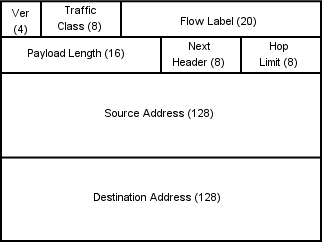
\includegraphics[width=4in]{IPv6_header}
\caption{L'en-tête IPv6}
\label{fig:IPv6}
\end{figure}

\begin{table}[htb]
\caption{Plages de valeurs pour le champ \texttt{DSCP}}
\centering
\begin{tabular}{|c|c|l|}
\hline\rowcolor[gray]{0.8}\color{black}
Plage & Valeurs & Règle d'assignation\\\hline
1 & xxxxx0 & Assignation par une norme de l'IANA\\\hline
2 & xxxx11 & Expérimentation/Usage local\\\hline
3 & xxxx01 & Expérimentation/Usage local (pourrait être jointe à la plage 1)\\\hline
\end{tabular}
\label{tab:RangesDSCP}
\end{table}

% On veut éviter que la figure et le tableau soient placés au-delà de la section courante.
% To prevent the figure and table from being positioned outside of the current section. 
\FloatBarrier


%%
%% OBJECTIFS DE RECHERCHE / RESEARCH OBJECTIVES
%%
\section{Objectifs de recherche}  % 0.5 page
Les objectifs de la recherche sont de concevoir un algorithme $O(n)$.


%%
%% PLAN DU MEMOIRE / THESIS OUTLINE
%%
\section{Plan du mémoire}  % 0.5 page

Voir la Figure~\ref{fig:Layers} pour plus de détails. 

\begin{figure}[htb]
\centering
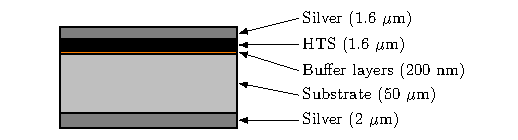
\includegraphics[width=4in]{demo_tikz}
\caption{Couches}
\label{fig:Layers}
\end{figure}


Un tableau : / A table:
\begin{table}[htb]
  \centering
  \caption{Constantes et variables du modèle analytique}
  \begin{tabular}{|c|l|}
    \hline\rowcolor[gray]{0.8}\color{black}
    Symbole         & Description\\\hline
    $\lambda$       & Taux d'arrivée moyen des requêtes de réservation de ressources\\\hline
    $\frac{1}{\mu}$ & Durée moyenne d'une session\\\hline
    $C$             & Capacité d'une cellule (nombre de sessions supportées)\\\hline
    $v_{moy}$       & Vitesse moyenne des MN dans le réseau d'accès\\\hline
    $L$             & Longueur d'un côté d'une cellule carrée\\\hline
    $n$             & Nombre moyen de MN dans une cellule\\\hline
    $\rho$          & Charge d'une cellule\\\hline
    $P_b$           & Probabilité de blocage d'une requête de réservation\\\hline
    $P_f$           & Probabilité d'interruption forcée d'une session\\\hline
    $P_c$           & Probabilité de compléter une session avec succès\\\hline
    $\Delta{}T$     & Délai de transmission\\\hline
  \end{tabular}
  \label{tab:Definitions}
\end{table}

La formule d'\mbox{Erlang-B}:
\begin{equation}
  P_b = \frac{\frac{\rho^C}{C!}}{\sum\limits_{x=0}^{C}\frac{\rho^x}{x!}}
  \label{eq:Pblock}
\end{equation}

Une autre équation : / Another equation:
\begin{equation}
  \begin{split}
    P_c &= (1 - P_b) \times (1 -  P_f)^N\\
        &= (1 - P_b)^{N+1}
  \end{split}
  \label{eq:ProbComplete}
\end{equation}

Enfin, l'expression suivante indique le moment à partir duquel les
réservations de ressources sont en place:
\begin{equation}
  \Delta{}T_{init} =
  \begin{cases}
    2\Delta{}T_{E2E} & \Delta{}T_{wan} > (\Delta{}T_{rad} + \Delta{}T_{net})\\
    \Delta{}T_{E2E} + 3(\Delta{}T_{rad} + \Delta{}T_{net}) & \text{sinon}
  \end{cases}
  \label{eq:InitCost}
\end{equation}

\paragraph{Le taux de paquets perdus} correspond au nombre de paquets
éliminés à cause d'une erreur de \emph{checksum} à un n\oe{}ud
quelconque ou d'une situation de congestion. Le taux de paquets perdus
pour un chemin est déterminé de la façon suivante:
\begin{equation}
  \label{eq:genPLR}
  PLR_P = 1 - \prod_{i=1}^N(1 - PLR_i)
\end{equation}

Toutefois, si les taux d'erreurs sont très faibles, comme c'est
généralement le cas pour des liens optiques, on peut approximer
$PLR_P$ de façon à le transformer en un paramètre additif:
\begin{equation}
  \label{eq:approxPLR}
  \begin{split}
    PLR_{L_1 \oplus L_2} &= 1 - (1 - PLR_1)(1 - PLR_2)\\
    &= 1 - (1 - PLR_2 - PLR_1 + \underbrace{PLR_1
      \times PLR_2}_\text{négligeable})\qquad PLR_1 \ll 1,
    PLR_2 \ll 1\\
    &\approx PLR_1 + PLR_2
  \end{split}
\end{equation}

\clearpage

Une courbe : / A curve:
\begin{figure}[htb]
\centering
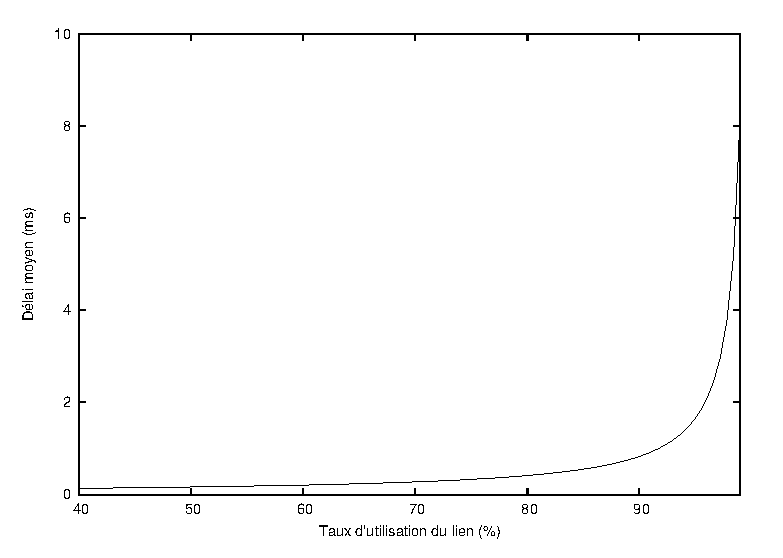
\includegraphics[width=5in]{LinkUsage}
\caption{Délai moyen en fonction du taux d'utilisation d'un lien}
\label{fig:LinkUse}
\end{figure}

\selectlanguage{english}
This paragraph is formatted by \LaTeX{} according to the standard rules of the
English language (\mbox{e.g.} hyphenation).
\selectlanguage{french}

L'arithmétique en virgule flottante peut entraîner des erreurs
d'approximation et il est important d'en être conscient
\cite{Rossi2011}.

De même, les calculs effectués sur une carte graphique (GPU) peuvent
introduire des erreurs d'approximation \cite{DeSantis2002, Cohen2006,
  Thorsson2014, Schirmer2012, Sakai2015, Electrical2006,
  Min2016, Massicotte2013, Kaliouby1987, Daintith2010, Haist2014, Kizza2013,
  Manasreh2011, Brydson1999, Boyce2002}.
       % Introduction au sujet de recherche.
\Chapter{REVUE DE LITTÉRATURE / LITERATURE REVIEW}\label{sec:RevLitt}
Texte / Text.

Voir la Figure~\ref{fig:Circuit} pour plus de détails. 

\begin{figure}[htb]
\centering
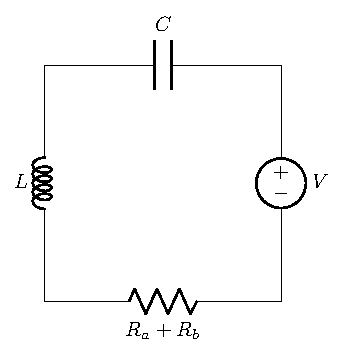
\includegraphics[width=2in]{Circuit_compile}
\caption{Circuit}
\label{fig:Circuit}
\end{figure}  % Revue de littérature / Literature review
\Chapter{PREMIER THÈME / FIRST THEME}\label{sec:Theme1}
Texte / Text.
             % Premier thème (Doctorat) ou "Détails de la Solution" (Maîtrise) / First topic (PhD) or "Details of the Solution" (Master's).
\Chapter{SECOND THÈME / SECOND THEME}\label{sec:Theme2}
Texte / Text.
             % Second thème (Doctorat) ou "Résultats théoriques et expérimentaux" (Maîtrise) / Second theme (PhD) or "Theoretical and experimental results" (Master's)
\Chapter{TROISIÈME THÈME AVEC UN TITRE TRÈS LONG QUI S'ÉTEND SUR DEUX LIGNES / THIRD THEME WITH A VERY LONG TITLE THAT EXTENDS ON TWO LINES}\label{sec:Theme3}

Lorem ipsum dolor sit amet, non faucibus ut, ante integer tristique odio
vitae turpis in. Euismod ullamcorper urna eget sollicitudin consectetuer,
dolor a. Ridiculus volutpat fusce, montes ipsum placerat, eu malesuada
maecenas a odio per, est pellentesque integer auctor sed ut sed, lectus
sodales orci ornare. Donec neque turpis vehicula. Duis vel sapien nec massa
lobortis nonummy. Feugiat ultrices urna mauris.

Potenti erat molestie ridiculus placerat, viverra ut felis porttitor,
rhoncus accumsan non, dui magna quam justo, ultrices massa ut phasellus
donec viverra mauris. Mauris a, dictumst risus a ornare velit nulla
ultricies, neque leo pellentesque, sit sed et suscipit excepteur
aenean. Venenatis sodales, odio nostra in id nobis scelerisque, venenatis
sociosqu gravida blandit orci pellentesque, tincidunt velit sed elementum
lacus pretium nunc, aenean vel dui id. Elit placerat id dui nunc mollis,
diam sapien porta, ipsam elit magna imperdiet amet, erat feugiat, et eros
morbi feugiat velit fringilla. Lacinia phasellus lacinia magna nunc sed, a
rhoncus, sem eget, dui aliquam sit sed leo beatae non, quisque justo
dignissim.

Torquent curabitur magnis nullam viverra scelerisque, per lacus pellentesque
vivamus, mauris aliquam sem lacus vivamus nullam porta. Vivamus donec
maecenas nunc orci massa, orci neque luctus leo non, mauris quis metus
sagittis. Voluptatibus gravida interdum. Magna duis nulla odio lacus fugiat
non. Magna fusce nunc, eget pellentesque nec. Imperdiet non magna
sollicitudin pellentesque, fusce erat interdum diam tellus vel, vitae
iaculis lectus varius suspendisse. Ac vel a in semper tellus, lobortis sed,
ipsum volutpat. Mauris a nunc aliquam metus nec, eu et id risus, diam
integer molestie suspendisse, sed wisi. Metus sed justo sodales sapien
molestie, suspendisse sem viverra ac proin, lorem luctus at tellus, velit mi
morbi orci in vestibulum, dignissim urna ornare id donec. Suspendisse non
enim euismod odio elit mauris, consectetuer pellentesque faucibus velit ante
lacinia sed.

Et dui erat. Wisi lorem eleifend cursus do donec, sed vel fermentum nec, a a
in pharetra. Ultricies risus, eget habitasse in, consectetuer metus in
auctor ac pellentesque curabitur, pulvinar aliquet eget. Mattis eget
venenatis dolor, nunc sem sed massa, urna scelerisque a magnis, neque elit
nec aliquam nonummy ac accusantium. Id vivamus nunc, erat justo tellus,
scelerisque habitasse accumsan tellus, pede sem vestibulum velit in et
eleifend. Nulla massa aenean integer dui. Suscipit nunc purus, rutrum velit,
mi torquent elementum in tincidunt. Maecenas nulla integer fringilla dapibus
tellus sit, enim amet magna eu erat, libero consectetuer nisl sapien, in
ultricies neque arcu sodales sagittis.

Lorem ipsum dolor sit amet, non faucibus ut, ante integer tristique odio
vitae turpis in. Euismod ullamcorper urna eget sollicitudin consectetuer,
dolor a. Ridiculus volutpat fusce, montes ipsum placerat, eu malesuada
maecenas a odio per, est pellentesque integer auctor sed ut sed, lectus
sodales orci ornare. Donec neque turpis vehicula. Duis vel sapien nec massa
lobortis nonummy. Feugiat ultrices urna mauris.

Potenti erat molestie ridiculus placerat, viverra ut felis porttitor,
rhoncus accumsan non, dui magna quam justo, ultrices massa ut phasellus
donec viverra mauris. Mauris a, dictumst risus a ornare velit nulla
ultricies, neque leo pellentesque, sit sed et suscipit excepteur
aenean. Venenatis sodales, odio nostra in id nobis scelerisque, venenatis
sociosqu gravida blandit orci pellentesque, tincidunt velit sed elementum
lacus pretium nunc, aenean vel dui id. Elit placerat id dui nunc mollis,
diam sapien porta, ipsam elit magna imperdiet amet, erat feugiat, et eros
morbi feugiat velit fringilla. Lacinia phasellus lacinia magna nunc sed, a
rhoncus, sem eget, dui aliquam sit sed leo beatae non, quisque justo
dignissim.

Torquent curabitur magnis nullam viverra scelerisque, per lacus pellentesque
vivamus, mauris aliquam sem lacus vivamus nullam porta. Vivamus donec
maecenas nunc orci massa, orci neque luctus leo non, mauris quis metus
sagittis. Voluptatibus gravida interdum. Magna duis nulla odio lacus fugiat
non. Magna fusce nunc, eget pellentesque nec. Imperdiet non magna
sollicitudin pellentesque, fusce erat interdum diam tellus vel, vitae
iaculis lectus varius suspendisse. Ac vel a in semper tellus, lobortis sed,
ipsum volutpat. Mauris a nunc aliquam metus nec, eu et id risus, diam
integer molestie suspendisse, sed wisi. Metus sed justo sodales sapien
molestie, suspendisse sem viverra ac proin, lorem luctus at tellus, velit mi
morbi orci in vestibulum, dignissim urna ornare id donec. Suspendisse non
enim euismod odio elit mauris, consectetuer pellentesque faucibus velit ante
lacinia sed.

Et dui erat. Wisi lorem eleifend cursus do donec, sed vel fermentum nec, a a
in pharetra. Ultricies risus, eget habitasse in, consectetuer metus in
auctor ac pellentesque curabitur, pulvinar aliquet eget. Mattis eget
venenatis dolor, nunc sem sed massa, urna scelerisque a magnis, neque elit
nec aliquam nonummy ac accusantium. Id vivamus nunc, erat justo tellus,
scelerisque habitasse accumsan tellus, pede sem vestibulum velit in et
eleifend. Nulla massa aenean integer dui. Suscipit nunc purus, rutrum velit,
mi torquent elementum in tincidunt. Maecenas nulla integer fringilla dapibus
tellus sit, enim amet magna eu erat, libero consectetuer nisl sapien, in
ultricies neque arcu sodales sagittis.

             % Troisième thème (Doctorat) ou effacez ce fichier si vous êtes à la Maîtrise / Third topic (PhD) or delete this file if you are in the Master's program
\Chapter{CONCLUSION}\label{sec:Conclusion}
Texte / Text.

%%
%%  SYNTHESE DES TRAVAUX / SUMMARY OF WORKS
%%
\section{Synthèse des travaux / Summary of Works}
Texte / Text.

%%
%%  LIMITATIONS
%%
\section{Limitations de la solution proposée / Limitations}\label{sec:Limitations}

%%
%%  AMELIORATIONS FUTURES / FUTURE RESEARCH
%%
\section{Améliorations futures / Future Research}
Texte / Text.
         % Conclusion.
%\backmatter
\ifthenelse{\equal{\Langue}{english}}{
	\renewcommand\bibname{REFERENCES}
	\bibliography{Document}
	\bibliographystyle{IEEEtran}			% Style bibliographique / Bibliography style 
}{
	\renewcommand\bibname{RÉFÉRENCES}
	\bibliography{Document}
	\bibliographystyle{IEEEtran-francais}    % Style bibliographique / Bibliography style 
}
%
\ifthenelse{\equal{\AnnexesPresentes}{O}}{
	\appendix%
	\newcommand{\Annexe}[1]{\annexe{#1}\setcounter{figure}{0}\setcounter{table}{0}\setcounter{footnote}{0}}%
	%%
%%  Annexes
%%
%%  Note: Ne pas modifier la ligne ci-dessous. / Do not modify the following line.
\ifthenelse{\equal{\Langue}{english}}{
	\addcontentsline{toc}{compteur}{APPENDICES}
}{
	\addcontentsline{toc}{compteur}{ANNEXES}
}
%%
%%
%%  Toutes les annexes doivent être inclues dans ce document
%%  les unes à la suite des autres.
%%  All annexes must be included in this document one after the other.
\Annexe{Démo}
Texte de l'annexe A\@. Remarquez que la phrase précédente se termine
par une lettre majuscule suivie d'un point. On indique explicitement
cette situation à \LaTeX{} afin que ce dernier ajuste correctement
l'espacement entre le point final de la phrase et le début de la
phrase suivante.


\begin{landscape}
\Annexe{Encore une annexe / Another Appendix}
Texte de l'annexe B\@ en mode «landscape».
\end{landscape}

\Annexe{Une dernière annexe / The Last Appendix}
Texte de l'annexe C\@.
}
{}
\end{document}
